\section{Module de croissance du zooplancton}

\subsection{Description du module}
\par{
In der vierten Aufgabenstellung geht es um die Vorhersage der Vermehrung von Phytoplankton in Abhängigkeit
von 
}

\begin{equation}
  {{d[DA]}\over{dt}} =
  \mu_{DA} [DA] - graz_{MSZ} [MSZ]
  \label{eq:partie1DiffEq1}
\end{equation}
\begin{equation}
  {{d[MSZ]}\over{dt}} =
  \left (
    (1- eges_{MSZ}) graz_{MSZ} Y_{MSZ} - mm_{MSZ}
  \right ) [MSZ]
  \label{eq:partie1DiffEq2}
\end{equation}

\begin{equation}
  graz_{MSZ} = g_{MSZ} \max(T) {{[DA]}\over{kg_{MSZ}+[DA]}}
  \label{eq:partie1GrazMic}
\end{equation}
\begin{equation}
  graz_{MSZ} = g_{MSZ} \max(T) {{[DA]-[DA_0]}\over{kg_{MSZ}+([DA]-[DA_0])}}
  \label{eq:partie1GrazMicSeul}
\end{equation}
\begin{equation}
  graz_{MSZ} = g_{MSZ} \max(T) {{[DA]^2}\over{kg_{MSZ}^2+[DA]^2}}
  \label{eq:partie1GrazHol}
\end{equation}

\begin{figure}
  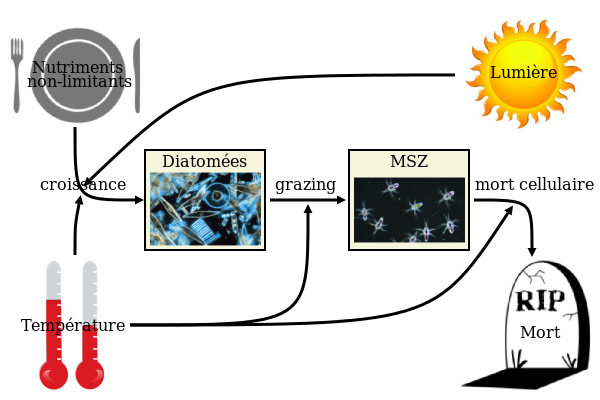
\includegraphics[width=\textwidth]{partie1/diagrammeConceptuel.png}
  \caption{Le modèle conceptuel du système étudié dans le quatrième cours.}
  \label{fig:partie1DiagConcept}
\end{figure}


\subsection{Analyse mathèmatique}
\subsubsection{États stationnaires}
\subsubsection{Stabilité des états stationnaires}

\subsection{Simulation de référence}

\subsection{Simulation de test 1}
